\chapter{Example Mission Scripts}

This chapter provides three progressively complex examples of mission scripts using DroneDSL. These scripts illustrate the computational capabilities of DroneDSL in the context of mission planning.

\section{Appendix 1}
This basic mission script tasks a drone with patrolling a specified area once, using the "coco" deep neural network model to detect objects during the patrol. It specifies waypoints, camera settings, and operational parameters to optimize the detection process.
\begin{lstlisting}[style=customgo]
Task {
    Detect task1 {
        way_points: [(-79.9502696,40.4156737,5.0),
                     (-79.9502655,40.4154588,5.0),
                     (-79.9499142,40.4154567,5.0),
                     (-79.9499128,40.4156753,5.0),
                     (-79.9502696,40.4156737,5.0)],
        gimbal_pitch: -20.0,
        drone_rotation: 0.0,
        sample_rate: 2,
        hover_delay: 0,
        model: coco,
    }
}

Mission {
    Start task1
}
\end{lstlisting}

\section{Appendix 2}
This script depicts a more complex surveillance mission, instructing the drone to alternate between patrolling a triangular and a rectangular area using the 'coco' model. If a car is detected, the drone begins a 20-second tracking task. The mission cycle repeats with transitions based on detection and tracking outcomes. The mission ends if a tracking task loses sight of its target for 10 seconds or a detection task completes without finding its target. The path followed is illustrated in \ref{fig:appendix_1}.
\begin{lstlisting}[style=customgo]
Task {
    Detect tri {
        way_points: <Triangle>,
        gimbal_pitch: -20.0,
        drone_rotation: 0.0,
        sample_rate: 2,
        hover_delay: 0,
        model: coco,
    }
    
    Detect rec {
        way_points: <Rectangle>,
        gimbal_pitch: -20.0,
        drone_rotation: 0.0,
        sample_rate: 2,
        hover_delay: 0,
        model: coco,
    }

    Track tri_track {
        gimbal_pitch: -30.0,
        model: coco,
        class: car,
    }
    
    Track rec_track {
        gimbal_pitch: -30.0,
        model: coco,
        class: car,
    }
}

Mission {
    Start tri
    Transition (object_detection(car)) tri -> tri_track
    Transition (timeout(20)) tri_track -> rec
    Transition (object_detection(car)) rec -> rec_track
    Transition (timeout(20)) rec_track -> tri
}
\end{lstlisting}

\begin{figure}[H]
    \centering
    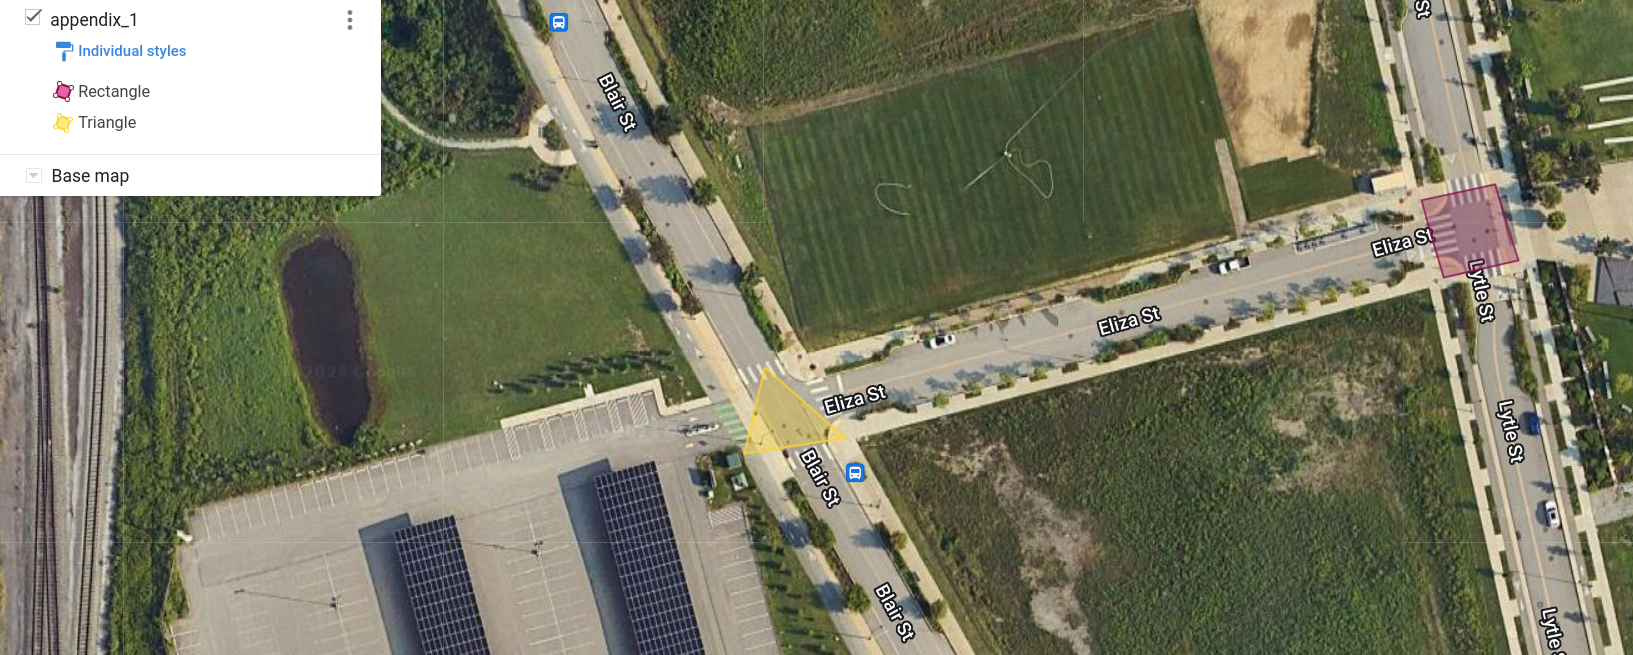
\includegraphics[width=0.8\textwidth]{Pictures/thesis_appendix_2.png}
    \caption{Illustrative Flight Route for Appendix 2.}
    \label{fig:appendix_1}
\end{figure}

\section{Appendix 3}
This mission script involves a drone navigating the Hot Metal Bridge while avoiding obstacles and subsequently monitoring pedestrian movement along the Three River Heritage Trail. Detection and tracking tasks use the 'midas' and 'visdrone' models respectively. The mission concludes when a pedestrian is out of sight for 10 seconds after being tracked. The trajectory of the mission is displayed in \ref{fig:appendix_2}.
\begin{lstlisting}[style=customgo]
Task {
    avoid task1 {
        way_points: <HotMetalBridge>
        speed: 1.0
        model: midas
        altitude: 8.0
    }

    Detect task2 {
        way_points: <ThreeRiverHerritageTrail>
        gimbal_pitch: -20.0,
        drone_rotation: 0.0,
        sample_rate: 2,
        hover_delay: 0,
        model: visdrone,
    }

    Track task3 {
        gimbal_pitch: -30.0,
        model: visdrone,
        class: pedestrian,
    }
}

Mission {
    Start task1
    Transition (object_detection(pedestrian)) task2 -> task3
    Transition (done) task2 -> task2
    Transition (done) task1 -> task2
}
\end{lstlisting}

\begin{figure}[H]
    \centering
    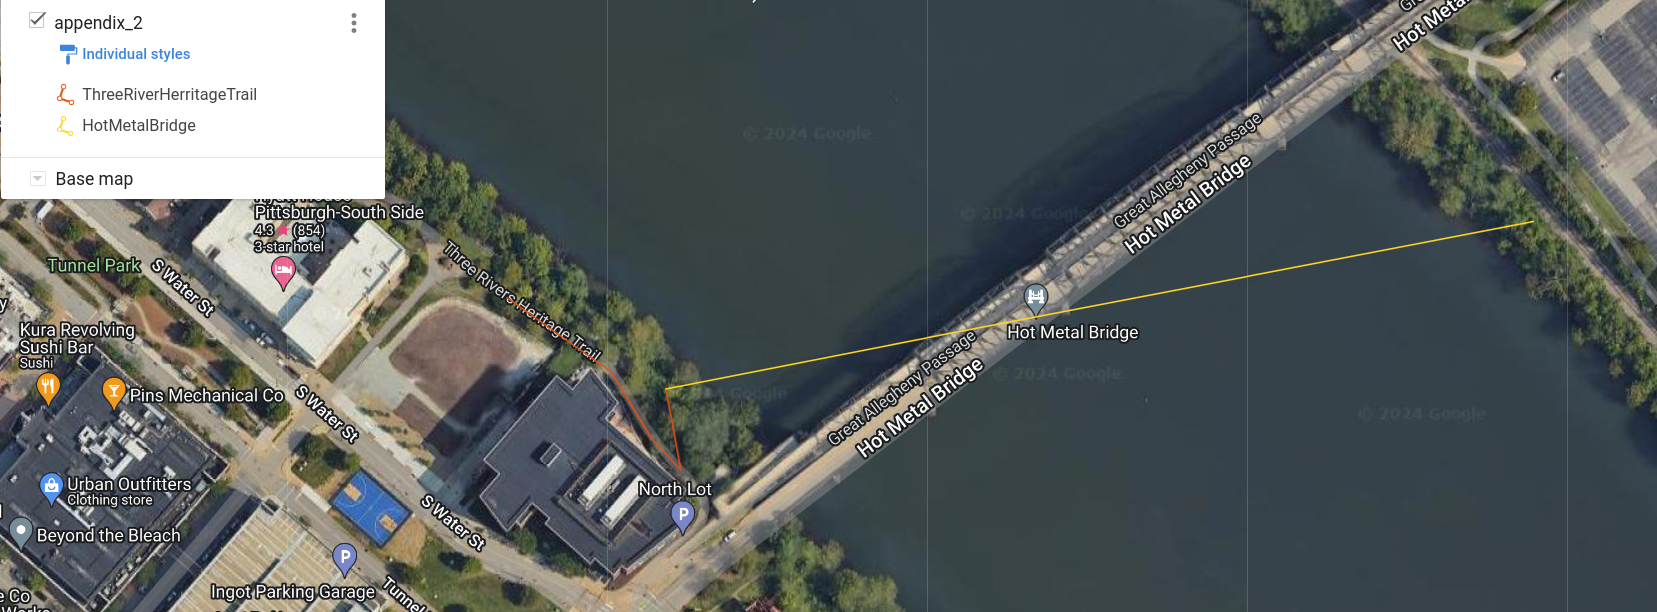
\includegraphics[width=0.8\textwidth]{Pictures/thesis_appendix_3.png}
    \caption{Flight Route for Appendix 3.}
    \label{fig:appendix_2}
\end{figure}